% !TeX program = pdflatex
% Template LaTeX para TCC de graduação da UNIPAMPA — V2
% Copyright (c) 2026 Charles Quevedo Carpes.
% Autoria das contribuições próprias, organização e adaptações do template.
% This work may be distributed and/or modified under the conditions of the
% LaTeX Project Public License, version 1.3c or (at your option) any later version.
% License: https://www.latex-project.org/lppl/lppl-1-3c.txt (see LICENSE).
% This work has the LPPL maintenance status `author-maintained'.
% The Current Maintainer of this work is Charles Quevedo Carpes.
% Consulte AUTORIA.md para escopo, créditos e relação dos arquivos.

% Compilador recomendado no Overleaf: pdfLaTeX (mais rápido no plano gratuito)
%Você também pode usar o textpage.com que também possui plano gratuito
% Para impressão em uma face:   \documentclass[anverso]{unipampa-tcc}
% Para impressão frente e verso:\documentclass[frente-verso]{unipampa-tcc}
\documentclass[anverso]{unipampa-tcc}

% Template LaTeX para TCC de graduação da UNIPAMPA — V2
% Copyright (c) 2026 Charles Quevedo Carpes.
% Autoria das contribuições próprias, organização e adaptações do template.
% This work may be distributed and/or modified under the conditions of the
% LaTeX Project Public License, version 1.3c or (at your option) any later version.
% License: https://www.latex-project.org/lppl/lppl-1-3c.txt (see LICENSE).
% This work has the LPPL maintenance status `author-maintained'.
% The Current Maintainer of this work is Charles Quevedo Carpes.
% Consulte AUTORIA.md para escopo, créditos e relação dos arquivos.

% =============================================================================
% DADOS DO TRABALHO - preencha apenas este arquivo
% =============================================================================

\instituicao{Universidade Federal do Pampa}
\campus{Campus (Nome do Campus)}
\curso{(Nome do Curso)}

\autor{Nome completo do autor}
\titulo{Título do trabalho}
\subtitulo{Subtítulo, se houver}

\local{Cidade}
\data{Ano}

% Titulação pretendida e campos acadêmicos
\grau{Licenciado em Matemática}
\areaconcentracao{Nome da área, se houver}
\linhapesquisa{}

% Texto da natureza do trabalho. Mantê-lo em espaço simples.
\preambulo{Trabalho de Conclusão de Curso apresentado ao Curso de (Nome do curso) da Universidade Federal do Pampa, como requisito parcial para obtenção do Título de Licenciado (ou Bacharel) em (Área do curso).}

\orientador{Prof. Dr. Nome completo do orientador}
% Deixe vazio quando não houver coorientador.
\coorientador{Nome do Coorientador}

\datadefesa{dia de mês de ano}

% Cada membro: nome e titulação; função; instituição.
\membrobanca{Prof. Dr. Nome completo do orientador}{Orientador}{Universidade Federal do Pampa}
\membrobanca{Profa. Dra. Nome do segundo membro}{Coorientador - Opcional}{Universidade Federal do Pampa}
\membrobanca{Prof. Dr. Nome do terceiro membro}{Instituição do membro}

% Logo é opcional e não é usado por padrão.
% \logo{figuras/logo-unipampa.pdf}

% Ficha catalográfica gerada no GURI. Enquanto o arquivo não existir, o template
% cria uma página de reserva. A ficha é excluída da contagem de páginas.
\arquivoFichaCatalografica{documentos/ficha-catalografica.pdf}

% Para o depósito final, é possível substituir a folha de aprovação editável por
% uma página assinada em PDF. Deixe comentado enquanto estiver redigindo.
% \arquivoFolhaAprovacao{documentos/folha-aprovacao-assinada.pdf}


\begin{document}

% =============================================================================
% PARTE EXTERNA E ELEMENTOS PRÉ-TEXTUAIS
% =============================================================================
\pretextual
\imprimircapa
\imprimirfolhaderosto
\inserirfichacatalografica
\imprimirfolhadeaprovacao

% Elementos opcionais: comente as linhas que não desejar utilizar.
% Template LaTeX para TCC de graduação da UNIPAMPA — V2
% Copyright (c) 2026 Charles Quevedo Carpes.
% Autoria das contribuições próprias, organização e adaptações do template.
% This work may be distributed and/or modified under the conditions of the
% LaTeX Project Public License, version 1.3c or (at your option) any later version.
% License: https://www.latex-project.org/lppl/lppl-1-3c.txt (see LICENSE).
% This work has the LPPL maintenance status `author-maintained'.
% The Current Maintainer of this work is Charles Quevedo Carpes.
% Consulte AUTORIA.md para escopo, créditos e relação dos arquivos.

\fazerDedicatoria{Dedico este trabalho à minha família, pelo apoio e incentivo durante toda a trajetória acadêmica.

(A dedicatória é opcional).
}

% Template LaTeX para TCC de graduação da UNIPAMPA — V2
% Copyright (c) 2026 Charles Quevedo Carpes.
% Autoria das contribuições próprias, organização e adaptações do template.
% This work may be distributed and/or modified under the conditions of the
% LaTeX Project Public License, version 1.3c or (at your option) any later version.
% License: https://www.latex-project.org/lppl/lppl-1-3c.txt (see LICENSE).
% This work has the LPPL maintenance status `author-maintained'.
% The Current Maintainer of this work is Charles Quevedo Carpes.
% Consulte AUTORIA.md para escopo, créditos e relação dos arquivos.

\begin{agradecimentostcc}
Agradeço ao meu orientador pelas contribuições, pela disponibilidade e pelo acompanhamento durante o desenvolvimento deste trabalho.

Agradeço aos professores, colegas, familiares e demais pessoas que contribuíram para minha formação acadêmica.

(O agradecimento é opcional)
\end{agradecimentostcc}

% Template LaTeX para TCC de graduação da UNIPAMPA — V2
% Copyright (c) 2026 Charles Quevedo Carpes.
% Autoria das contribuições próprias, organização e adaptações do template.
% This work may be distributed and/or modified under the conditions of the
% LaTeX Project Public License, version 1.3c or (at your option) any later version.
% License: https://www.latex-project.org/lppl/lppl-1-3c.txt (see LICENSE).
% This work has the LPPL maintenance status `author-maintained'.
% The Current Maintainer of this work is Charles Quevedo Carpes.
% Consulte AUTORIA.md para escopo, créditos e relação dos arquivos.

\fazerEpigrafe{Uma citação breve e relacionada ao tema do trabalho.}{Autor da citação
 
 (A epígrafe é opcional)}


% Elementos obrigatórios
% Template LaTeX para TCC de graduação da UNIPAMPA — V2
% Copyright (c) 2026 Charles Quevedo Carpes.
% Autoria das contribuições próprias, organização e adaptações do template.
% This work may be distributed and/or modified under the conditions of the
% LaTeX Project Public License, version 1.3c or (at your option) any later version.
% License: https://www.latex-project.org/lppl/lppl-1-3c.txt (see LICENSE).
% This work has the LPPL maintenance status `author-maintained'.
% The Current Maintainer of this work is Charles Quevedo Carpes.
% Consulte AUTORIA.md para escopo, créditos e relação dos arquivos.

\begin{resumotcc}
Este arquivo deve conter um resumo informativo, redigido em terceira pessoa, em parágrafo único e com extensão entre 150 e 500 palavras. O texto deve apresentar, de maneira concisa, o tema, o objetivo, a metodologia, os principais resultados e as considerações finais do Trabalho de Conclusão de Curso. Evitam-se enumerações, citações, fórmulas, símbolos e abreviaturas pouco conhecidas. Substitua este texto pelo resumo definitivo e confira a correspondência integral entre a versão em português e o resumo em língua estrangeira.

\palavraschave{normalização acadêmica; trabalho de conclusão de curso; Universidade Federal do Pampa; LaTeX}
\end{resumotcc}

% Template LaTeX para TCC de graduação da UNIPAMPA — V2
% Copyright (c) 2026 Charles Quevedo Carpes.
% Autoria das contribuições próprias, organização e adaptações do template.
% This work may be distributed and/or modified under the conditions of the
% LaTeX Project Public License, version 1.3c or (at your option) any later version.
% License: https://www.latex-project.org/lppl/lppl-1-3c.txt (see LICENSE).
% This work has the LPPL maintenance status `author-maintained'.
% The Current Maintainer of this work is Charles Quevedo Carpes.
% Consulte AUTORIA.md para escopo, créditos e relação dos arquivos.

\begin{abstracttcc}
This file must contain the full foreign-language version of the abstract, written as a single paragraph. It should accurately reproduce the objective, methodology, main results, and final considerations presented in the Portuguese abstract. Replace this sample with the definitive text and review technical terminology carefully.

\keywords{academic standardization; undergraduate thesis; Federal University of Pampa; LaTeX}
\end{abstracttcc}


% Listas opcionais. Use apenas quando houver elementos correspondentes.
\pdfbookmark[0]{LISTA DE FIGURAS}{lof}
\renewcommand{\listfigurename}{LISTA DE FIGURAS}
\listoffigures*
\clearpage

\pdfbookmark[0]{LISTA DE TABELAS}{lot}
\renewcommand{\listtablename}{LISTA DE TABELAS}
\listoftables*
\clearpage

% \listadequadros
% Template LaTeX para TCC de graduação da UNIPAMPA — V2
% Copyright (c) 2026 Charles Quevedo Carpes.
% Autoria das contribuições próprias, organização e adaptações do template.
% This work may be distributed and/or modified under the conditions of the
% LaTeX Project Public License, version 1.3c or (at your option) any later version.
% License: https://www.latex-project.org/lppl/lppl-1-3c.txt (see LICENSE).
% This work has the LPPL maintenance status `author-maintained'.
% The Current Maintainer of this work is Charles Quevedo Carpes.
% Consulte AUTORIA.md para escopo, créditos e relação dos arquivos.

\begin{listadeabreviaturas}
  \item[n.] número
  \item[p.] página
  \item[f.] folha
  \item[cap.] capítulo
\end{listadeabreviaturas}

% Template LaTeX para TCC de graduação da UNIPAMPA — V2
% Copyright (c) 2026 Charles Quevedo Carpes.
% Autoria das contribuições próprias, organização e adaptações do template.
% This work may be distributed and/or modified under the conditions of the
% LaTeX Project Public License, version 1.3c or (at your option) any later version.
% License: https://www.latex-project.org/lppl/lppl-1-3c.txt (see LICENSE).
% This work has the LPPL maintenance status `author-maintained'.
% The Current Maintainer of this work is Charles Quevedo Carpes.
% Consulte AUTORIA.md para escopo, créditos e relação dos arquivos.

\begin{listadesiglas}
  \item[ABNT] Associação Brasileira de Normas Técnicas
  \item[TCC] Trabalho de Conclusão de Curso
  \item[HTML] Hypertext Markup Language
\end{listadesiglas}


% % Template LaTeX para TCC de graduação da UNIPAMPA — V2
% Copyright (c) 2026 Charles Quevedo Carpes.
% Autoria das contribuições próprias, organização e adaptações do template.
% This work may be distributed and/or modified under the conditions of the
% LaTeX Project Public License, version 1.3c or (at your option) any later version.
% License: https://www.latex-project.org/lppl/lppl-1-3c.txt (see LICENSE).
% This work has the LPPL maintenance status `author-maintained'.
% The Current Maintainer of this work is Charles Quevedo Carpes.
% Consulte AUTORIA.md para escopo, créditos e relação dos arquivos.

\begin{listadesimbolos}
  \item[$\sigma$] Desvio padrão
  \item[$\Delta t$] Variação de tempo
\end{listadesimbolos}


\sumariotcc

% =============================================================================
% ELEMENTOS TEXTUAIS
% =============================================================================
\iniciotextual
% Template LaTeX para TCC de graduação da UNIPAMPA — V2
% Copyright (c) 2026 Charles Quevedo Carpes.
% Autoria das contribuições próprias, organização e adaptações do template.
% This work may be distributed and/or modified under the conditions of the
% LaTeX Project Public License, version 1.3c or (at your option) any later version.
% License: https://www.latex-project.org/lppl/lppl-1-3c.txt (see LICENSE).
% This work has the LPPL maintenance status `author-maintained'.
% The Current Maintainer of this work is Charles Quevedo Carpes.
% Consulte AUTORIA.md para escopo, créditos e relação dos arquivos.

\chapter{INTRODUÇÃO}

A introdução apresenta o tema, a delimitação do estudo, o problema de pesquisa, a justificativa, os objetivos, uma síntese da metodologia e a organização do trabalho.

Este template adota o sistema autor-data. Uma citação indireta pode ser apresentada de modo narrativo, como em \citeonline{gil2022}, ou ao final da sentença \cite{gil2022}. A indicação de página em citações indiretas é opcional. Para maiores informações ou em caso de dúvidas deve ser  consultado o \textbf{Manual de Citações} disponível em: \url{https://sites.unipampa.edu.br/sisbi/files/2025/07/manual-de-normalizacao-de-citacao-sistema-de-chamada-e-notas-2025.pdf}


Para que as referências apareçam na seção correta, no final do texto, é necessário que elas tenham sido citadas em algum lugar do TCC. Vamos inserir uma frase aqui que cita todas as referências que temos no arquivo .bib que desse template. Isso fará o compilador inserir todas nas referências.

Estudos diversos abrangem áreas como literatura \cite{alves2000}, engenharia e tubulações \cite{bailona2006}, legislação federal \cite{brasil1988, brasil2024}, assessoria educacional \cite{cassol2003}, avaliação de revestimentos \cite{courtes2018}, auditoria bancária \cite{dantas2014}, jornalismo digital \cite{ferreira2003}, metodologia da pesquisa \cite{gil2022, ruiz2008}, teorias da personalidade \cite{hall2000}, redes de computadores \cite{jonack2006}, economia e globalização \cite{lacerda1998, mariano2005}, métodos educacionais \cite{capitulo2024}, tecnologias no ensino \cite{artigo2025}, pós-graduação \cite{dissertacao2023}, automação acadêmica \cite{evento2024}, normas técnicas \cite{abnt14724, unipampa2025manual}, biblioteconomia \cite{silva2012}, serviço social \cite{simoes2009}, softwares de apoio \cite{software2026}, diário oficial \cite{brasil1988}.

\section{Problema de pesquisa}

Apresente a pergunta que orienta a investigação de forma clara, delimitada e coerente com os objetivos.

\section{Objetivos}

\subsection{Objetivo geral}

Descreva o resultado principal que o trabalho pretende alcançar.

\subsection{Objetivos específicos}

Os objetivos específicos podem ser apresentados em alíneas:

\begin{alineas}
  \item identificar os elementos relevantes do problema;
  \item analisar os dados coletados;
  \item comparar os resultados obtidos; e
  \item apresentar as considerações finais.
\end{alineas}

\section{Organização do trabalho}

Explique brevemente o conteúdo das seções seguintes.

% Template LaTeX para TCC de graduação da UNIPAMPA — V2
% Copyright (c) 2026 Charles Quevedo Carpes.
% Autoria das contribuições próprias, organização e adaptações do template.
% This work may be distributed and/or modified under the conditions of the
% LaTeX Project Public License, version 1.3c or (at your option) any later version.
% License: https://www.latex-project.org/lppl/lppl-1-3c.txt (see LICENSE).
% This work has the LPPL maintenance status `author-maintained'.
% The Current Maintainer of this work is Charles Quevedo Carpes.
% Consulte AUTORIA.md para escopo, créditos e relação dos arquivos.

\chapter{REFERENCIAL TEÓRICO}

O referencial teórico reúne e discute a literatura relacionada ao problema investigado. Todas as fontes citadas no texto devem aparecer nas referências, e a lista final deve conter somente os documentos efetivamente citados.

\section{Citações diretas e indiretas}

Citações diretas de até três linhas permanecem no corpo do parágrafo, entre aspas duplas. Por exemplo: \enquote{a pesquisa científica exige planejamento e sistematização} \cite[p.~25]{gil2022}.

A citação direta com mais de três linhas deve ser apresentada sem aspas, com recuo de 4 cm, fonte 10 e espaçamento simples:

\begin{citacaodireta}
A citação longa é destacada do texto e deve reproduzir fielmente o trecho consultado. A chamada autor-data inclui o sobrenome em letras maiúsculas e minúsculas, o ano e a página ou localização da fonte consultada \cite[p.~88]{hall2000}.
\end{citacaodireta}

Supressões são indicadas por \texttt{[...]}; acréscimos ou comentários, por colchetes; e destaques acrescentados pelo autor do TCC devem ser identificados com a expressão \enquote{grifo nosso} na chamada.

\section{Citação de citação}

A citação de citação deve ser utilizada somente quando o documento original não puder ser consultado. O pacote oferece os comandos \verb|\apud| e \verb|\apudonline|. Exemplo: \apud[p.~89]{lacerda1998}{mariano2005}.

\section{Notas de rodapé}

Notas explicativas devem ser utilizadas com moderação e não podem interromper a sequência lógica do texto.\footnote{Exemplo de nota explicativa em fonte 10, espaço simples e alinhamento suspenso.}

% Template LaTeX para TCC de graduação da UNIPAMPA — V2
% Copyright (c) 2026 Charles Quevedo Carpes.
% Autoria das contribuições próprias, organização e adaptações do template.
% This work may be distributed and/or modified under the conditions of the
% LaTeX Project Public License, version 1.3c or (at your option) any later version.
% License: https://www.latex-project.org/lppl/lppl-1-3c.txt (see LICENSE).
% This work has the LPPL maintenance status `author-maintained'.
% The Current Maintainer of this work is Charles Quevedo Carpes.
% Consulte AUTORIA.md para escopo, créditos e relação dos arquivos.

\chapter{METODOLOGIA}

Descreva a natureza e a abordagem da pesquisa, o delineamento, o local, os participantes ou a amostra, os instrumentos, os procedimentos de coleta e análise e, quando aplicável, os cuidados éticos.

\section{Exemplo de ilustração}

Toda ilustração deve ser citada no texto e inserida o mais próximo possível da passagem a que se refere. A Figura~\ref{fig:fluxo} apresenta um exemplo criado diretamente em LaTeX.

\begin{figure}[H]
  \caption{Fluxo simplificado das etapas da pesquisa}
  \label{fig:fluxo}
  \centering
  \setlength{\fboxsep}{10pt}
  \fbox{\begin{minipage}{0.82\textwidth}
    \centering
    Definição do problema $\longrightarrow$ Coleta de dados $\longrightarrow$ Análise $\longrightarrow$ Resultados
  \end{minipage}}
  \fonte{elaboração própria}
\end{figure}

A Figura~\ref{fig:fluxo2} apresenta um exemplo de imagem jpg inserida no texto.

\begin{figure}[H]
  \caption{Exemplo de figura jpg inserida no texto}
  \label{fig:fluxo2}
  \centering
  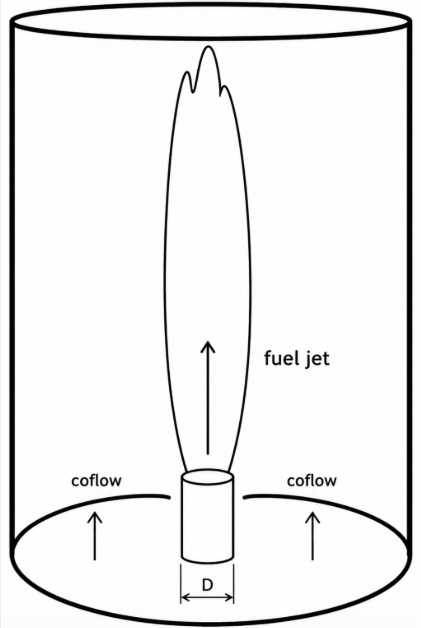
\includegraphics[width=0.82\textwidth]{figuras/fig1.jpg}
  \fonte{elaboração própria}
\end{figure}

\section{Exemplo de tabela}

As tabelas privilegiam dados numéricos e não devem apresentar linhas verticais. A Tabela~\ref{tab:exemplo} ilustra a apresentação recomendada.

\begin{table}[H]
  \caption{Distribuição hipotética dos participantes por grupo}
  \label{tab:exemplo}
  \centering
  \begin{tabular}{lrr}
    \toprule
    Grupo & Frequência & Percentual (\%) \\
    \midrule
    Grupo A & 18 & 45,0 \\
    Grupo B & 22 & 55,0 \\
    \midrule
    Total & 40 & 100,0 \\
    \bottomrule
  \end{tabular}
  \fonte{elaboração própria}
  \notatabela{valores apresentados apenas para demonstrar a formatação}
\end{table}

\section{Equações e fórmulas}

Equações podem ser destacadas e numeradas à direita. A Equação~\eqref{eq:media} apresenta a média aritmética:

\begin{equation}
  \bar{x}=\frac{1}{n}\sum_{i=1}^{n}x_i.
  \label{eq:media}
\end{equation}

A seguir outros exemplos de equações:


% ============================================================================
% SEÇÃO 1: EQUAÇÕES BÁSICAS E FUNDAMENTAIS
% ============================================================================

\section{Equações Básicas e Fundamentais}

\subsection{Identidades Clássicas}

Equação de Euler:
\begin{equation}
e^{i\pi} + 1 = 0
\end{equation}

Identidade trigonométrica fundamental:
\begin{equation}
\sin^2(x) + \cos^2(x) = 1
\end{equation}

Teorema de Pitágoras:
\begin{equation}
a^2 + b^2 = c^2
\end{equation}

Equação quadrática:
\begin{equation}
x = \frac{-b \pm \sqrt{b^2 - 4ac}}{2a}
\end{equation}

% ============================================================================
% SEÇÃO 2: CÁLCULO E ANÁLISE
% ============================================================================

\section{Cálculo e Análise}

\subsection{Limites}

\begin{equation}
\lim_{x \to \infty} \frac{1}{x} = 0
\end{equation}

\subsection{Derivadas}

Definição de derivada:
\begin{equation}
\frac{df}{dx} = \lim_{h \to 0} \frac{f(x+h) - f(x)}{h}
\end{equation}

Derivada parcial:
\begin{equation}
\frac{\partial u}{\partial t} + \frac{\partial u}{\partial x} = 0
\end{equation}

\subsection{Integrais}

Integral definida:
\begin{equation}
\int_a^b f(x)\,dx = F(b) - F(a)
\end{equation}

Integral dupla:
\begin{equation}
\iint_D f(x,y)\,dA
\end{equation}

Integral tripla:
\begin{equation}
\iiint_V f(x,y,z)\,dV
\end{equation}

\subsection{Séries}

Série de Taylor:
\begin{equation}
f(x) = \sum_{n=0}^{\infty} \frac{f^{(n)}(a)}{n!}(x-a)^n
\end{equation}

Série de Fourier:
\begin{equation}
f(x) = \frac{a_0}{2} + \sum_{n=1}^{\infty} \left[a_n \cos\left(\frac{n\pi x}{L}\right) + b_n \sin\left(\frac{n\pi x}{L}\right)\right]
\end{equation}

% ============================================================================
% SEÇÃO 3: ESTATÍSTICA E PROBABILIDADE
% ============================================================================

\section{Estatística e Probabilidade}

\subsection{Medidas Estatísticas}

Média aritmética:
\begin{equation}
\bar{x} = \frac{1}{n}\sum_{i=1}^{n} x_i
\end{equation}

Variância:
\begin{equation}
\sigma^2 = \frac{1}{n}\sum_{i=1}^{n}(x_i - \bar{x})^2
\end{equation}

Desvio padrão:
\begin{equation}
\sigma = \sqrt{\frac{1}{n}\sum_{i=1}^{n}(x_i - \mu)^2}
\end{equation}

Coeficiente de variação:
\begin{equation}
CV = \frac{\sigma}{\bar{x}} \times 100\%
\end{equation}

Coeficiente de correlação de Pearson:
\begin{equation}
r = \frac{\sum_{i=1}^{n}(x_i - \bar{x})(y_i - \bar{y})}{\sqrt{\sum_{i=1}^{n}(x_i - \bar{x})^2}\sqrt{\sum_{i=1}^{n}(y_i - \bar{y})^2}}
\end{equation}

\subsection{Distribuições de Probabilidade}

Distribuição normal:
\begin{equation}
f(x) = \frac{1}{\sigma\sqrt{2\pi}} \exp\left(-\frac{(x-\mu)^2}{2\sigma^2}\right)
\end{equation}

Distribuição de Poisson:
\begin{equation}
P(X=k) = \frac{\lambda^k e^{-\lambda}}{k!}
\end{equation}

Distribuição binomial:
\begin{equation}
P(X=k) = \binom{n}{k}p^k(1-p)^{n-k}
\end{equation}

\subsection{Tópicos de Probabilidade}

Teorema de Bayes:
\begin{equation}
P(A|B) = \frac{P(B|A)P(A)}{P(B)}
\end{equation}

Esperança matemática:
\begin{equation}
E[X] = \sum_{i} x_i P(X=x_i)
\end{equation}

Covariância:
\begin{equation}
\text{Cov}(X,Y) = E[(X - E[X])(Y - E[Y])]
\end{equation}

% ============================================================================
% SEÇÃO 4: FÍSICA CLÁSSICA
% ============================================================================

\section{Física Clássica}

Segunda lei de Newton:
\begin{equation}
F = ma
\end{equation}

Lei da gravitação universal:
\begin{equation}
F = G\frac{m_1 m_2}{r^2}
\end{equation}

Energia cinética:
\begin{equation}
E_k = \frac{1}{2}mv^2
\end{equation}

Energia potencial gravitacional:
\begin{equation}
E_p = mgh
\end{equation}

Teorema trabalho-energia:
\begin{equation}
W = \Delta E_k = \frac{1}{2}m(v_f^2 - v_i^2)
\end{equation}

Lei de Ohm:
\begin{equation}
V = IR
\end{equation}

Lei de Coulomb:
\begin{equation}
F = k\frac{q_1 q_2}{r^2}
\end{equation}

Potência:
\begin{equation}
P = \frac{W}{t} = \frac{dE}{dt}
\end{equation}

Momento linear:
\begin{equation}
\vec{p} = m\vec{v}
\end{equation}

Momento angular:
\begin{equation}
\vec{L} = \vec{r} \times \vec{p} = I\omega
\end{equation}

% ============================================================================
% SEÇÃO 5: FÍSICA MODERNA
% ============================================================================

\section{Física Moderna}

Equivalência massa-energia (Einstein):
\begin{equation}
E = mc^2
\end{equation}

Equação de Schrödinger independente do tempo:
\begin{equation}
-\frac{\hbar^2}{2m}\nabla^2\psi + V\psi = E\psi
\end{equation}

Equação de Schrödinger dependente do tempo:
\begin{equation}
i\hbar\frac{\partial\psi}{\partial t} = -\frac{\hbar^2}{2m}\nabla^2\psi + V\psi
\end{equation}

Relação de de Broglie:
\begin{equation}
\lambda = \frac{h}{p} = \frac{h}{mv}
\end{equation}

Princípio da incerteza de Heisenberg:
\begin{equation}
\Delta x \cdot \Delta p \geq \frac{\hbar}{2}
\end{equation}

Energia relativística:
\begin{equation}
E = \sqrt{(pc)^2 + (mc^2)^2}
\end{equation}

% ============================================================================
% SEÇÃO 6: ELETROMAGNETISMO
% ============================================================================

\section{Eletromagnetismo}

\subsection{Equações de Maxwell}

Lei de Gauss:
\begin{equation}
\oint \vec{E} \cdot d\vec{A} = \frac{Q}{\epsilon_0}
\end{equation}

Lei de Gauss para o magnetismo:
\begin{equation}
\oint \vec{B} \cdot d\vec{A} = 0
\end{equation}

Lei de Faraday:
\begin{equation}
\oint \vec{E} \cdot d\vec{l} = -\frac{d\Phi_B}{dt}
\end{equation}

Lei de Ampère-Maxwell:
\begin{equation}
\oint \vec{B} \cdot d\vec{l} = \mu_0\left(I + \epsilon_0\frac{d\Phi_E}{dt}\right)
\end{equation}

\subsection{Outras Leis do Eletromagnetismo}

Força de Lorentz:
\begin{equation}
\vec{F} = q(\vec{E} + \vec{v} \times \vec{B})
\end{equation}

Densidade de energia eletromagnética:
\begin{equation}
u = \frac{1}{2}\left(\epsilon_0 E^2 + \frac{B^2}{\mu_0}\right)
\end{equation}

Vetor de Poynting:
\begin{equation}
\vec{S} = \frac{1}{\mu_0}(\vec{E} \times \vec{B})
\end{equation}

% ============================================================================
% SEÇÃO 7: QUÍMICA
% ============================================================================

\section{Química}

Lei ideal dos gases:
\begin{equation}
PV = nRT
\end{equation}

Concentração molar:
\begin{equation}
c = \frac{n}{V}
\end{equation}

pH:
\begin{equation}
\text{pH} = -\log_{10}[H^+]
\end{equation}

Equação de Nernst:
\begin{equation}
E = E^0 - \frac{RT}{nF}\ln Q
\end{equation}

Constante de equilíbrio:
\begin{equation}
K_c = \frac{[C]^c[D]^d}{[A]^a[B]^b}
\end{equation}

Equação de Arrhenius:
\begin{equation}
k = A e^{-E_a/RT}
\end{equation}

Forma logarítmica de Arrhenius:
\begin{equation}
\ln(k) = \ln(A) - \frac{E_a}{RT}
\end{equation}

Entalpia de reação:
\begin{equation}
\Delta H_{rxn} = \sum \Delta H_f^\circ(\text{produtos}) - \sum \Delta H_f^\circ(\text{reagentes})
\end{equation}

Energia livre de Gibbs:
\begin{equation}
\Delta G = \Delta H - T\Delta S
\end{equation}

% ============================================================================
% SEÇÃO 8: ÁLGEBRA LINEAR
% ============================================================================

\section{Álgebra Linear}

\subsection{Determinantes}

Determinante de matriz 2×2:
\begin{equation}
\begin{vmatrix}
a & b \\
c & d
\end{vmatrix} = ad - bc
\end{equation}

Determinante de matriz 3×3:
\begin{equation}
\begin{vmatrix}
a & b & c \\
d & e & f \\
g & h & i
\end{vmatrix} = aei + bfg + cdh - ceg - afh - bdi
\end{equation}

\subsection{Operações com Vetores}

Produto escalar:
\begin{equation}
\vec{a} \cdot \vec{b} = |\vec{a}||\vec{b}|\cos\theta = \sum_{i=1}^{n} a_i b_i
\end{equation}

Produto vetorial:
\begin{equation}
\vec{a} \times \vec{b} = \begin{vmatrix}
\vec{i} & \vec{j} & \vec{k} \\
a_1 & a_2 & a_3 \\
b_1 & b_2 & b_3
\end{vmatrix}
\end{equation}

Norma de um vetor:
\begin{equation}
\|\vec{v}\| = \sqrt{v_1^2 + v_2^2 + \cdots + v_n^2}
\end{equation}

Ângulo entre vetores:
\begin{equation}
\cos\theta = \frac{\vec{a} \cdot \vec{b}}{|\vec{a}||\vec{b}|}
\end{equation}

\subsection{Operações com Matrizes}

Multiplicação de matrizes:
\begin{equation}
(AB)_{ij} = \sum_{k=1}^{n} a_{ik}b_{kj}
\end{equation}

Matriz inversa:
\begin{equation}
A^{-1} = \frac{1}{\det(A)} \text{adj}(A)
\end{equation}

Autovalor e autovetor:
\begin{equation}
A\vec{v} = \lambda\vec{v}
\end{equation}

Polinômio característico:
\begin{equation}
\det(A - \lambda I) = 0
\end{equation}

Traço de uma matriz:
\begin{equation}
\text{tr}(A) = \sum_{i=1}^{n} a_{ii}
\end{equation}

% ============================================================================
% SEÇÃO 9: EQUAÇÕES DIFERENCIAIS
% ============================================================================

\section{Equações Diferenciais}

\subsection{Equações Diferenciais Ordinárias}

Equação diferencial linear de primeira ordem:
\begin{equation}
\frac{dy}{dx} + P(x)y = Q(x)
\end{equation}

Equação diferencial linear homogênea de segunda ordem:
\begin{equation}
\frac{d^2y}{dx^2} + p(x)\frac{dy}{dx} + q(x)y = 0
\end{equation}

Equação diferencial de Bernoulli:
\begin{equation}
\frac{dy}{dx} + P(x)y = Q(x)y^n
\end{equation}

\subsection{Equações Diferenciais Parciais}

Equação de Laplace:
\begin{equation}
\nabla^2 u = \frac{\partial^2 u}{\partial x^2} + \frac{\partial^2 u}{\partial y^2} + \frac{\partial^2 u}{\partial z^2} = 0
\end{equation}

Equação de Poisson:
\begin{equation}
\nabla^2 u = f(x,y,z)
\end{equation}

Equação de calor/difusão:
\begin{equation}
\frac{\partial u}{\partial t} = \alpha \nabla^2 u
\end{equation}

Equação de onda:
\begin{equation}
\frac{\partial^2 u}{\partial t^2} = c^2 \nabla^2 u
\end{equation}

Equação de Burgers:
\begin{equation}
\frac{\partial u}{\partial t} + u\frac{\partial u}{\partial x} = \nu\frac{\partial^2 u}{\partial x^2}
\end{equation}

% ============================================================================
% SEÇÃO 10: SÉRIES E SOMATÓRIOS
% ============================================================================

\section{Séries e Somatórios}

\subsection{Séries Importantes}

Série geométrica:
\begin{equation}
\sum_{n=0}^{\infty} r^n = \frac{1}{1-r}, \quad |r| < 1
\end{equation}

Série harmônica:
\begin{equation}
\sum_{n=1}^{\infty} \frac{1}{n} = \infty
\end{equation}

Série p:
\begin{equation}
\sum_{n=1}^{\infty} \frac{1}{n^p} \text{ converge se } p > 1
\end{equation}

Série de potências:
\begin{equation}
\sum_{n=0}^{\infty} a_n(x-a)^n
\end{equation}

\subsection{Operadores de Somatória}

Somatório duplo:
\begin{equation}
\sum_{i=1}^{m} \sum_{j=1}^{n} a_{ij}
\end{equation}

Produtório:
\begin{equation}
\prod_{i=1}^{n} a_i = a_1 \cdot a_2 \cdot \ldots \cdot a_n
\end{equation}

Somatório telescópico:
\begin{equation}
\sum_{k=1}^{n} (a_{k+1} - a_k) = a_{n+1} - a_1
\end{equation}

% ============================================================================
% SEÇÃO 11: FUNÇÕES ESPECIAIS
% ============================================================================

\section{Funções Especiais e Transcendentais}

Identidades logarítmicas:
\begin{equation}
\ln(xy) = \ln(x) + \ln(y)
\end{equation}

\begin{equation}
\ln\left(\frac{x}{y}\right) = \ln(x) - \ln(y)
\end{equation}

Identidades exponenciais:
\begin{equation}
e^{x+y} = e^x \cdot e^y
\end{equation}

Função erro:
\begin{equation}
\text{erf}(x) = \frac{2}{\sqrt{\pi}}\int_0^x e^{-t^2}\,dt
\end{equation}

Função gama:
\begin{equation}
\Gamma(n) = \int_0^{\infty} t^{n-1}e^{-t}\,dt = (n-1)!
\end{equation}

Função beta:
\begin{equation}
B(x,y) = \int_0^1 t^{x-1}(1-t)^{y-1}\,dt
\end{equation}

Relação entre funções beta e gama:
\begin{equation}
B(x,y) = \frac{\Gamma(x)\Gamma(y)}{\Gamma(x+y)}
\end{equation}

Função de Bessel:
\begin{equation}
J_n(x) = \sum_{m=0}^{\infty} \frac{(-1)^m}{m!(n+m)!}\left(\frac{x}{2}\right)^{n+2m}
\end{equation}

% ============================================================================
% SEÇÃO 12: SISTEMAS DE EQUAÇÕES
% ============================================================================

\section{Sistemas de Equações}

\subsection{Sistemas Lineares}

Sistema 2×2:
\begin{equation}
\begin{cases}
a_1x + b_1y = c_1 \\
a_2x + b_2y = c_2
\end{cases}
\end{equation}

Forma matricial:
\begin{equation}
\begin{pmatrix}
a_{11} & a_{12} & \cdots & a_{1n} \\
a_{21} & a_{22} & \cdots & a_{2n} \\
\vdots & \vdots & \ddots & \vdots \\
a_{m1} & a_{m2} & \cdots & a_{mn}
\end{pmatrix}
\begin{pmatrix}
x_1 \\ x_2 \\ \vdots \\ x_n
\end{pmatrix}
=
\begin{pmatrix}
b_1 \\ b_2 \\ \vdots \\ b_m
\end{pmatrix}
\end{equation}

Regra de Cramer:
\begin{equation}
x_i = \frac{\det(A_i)}{\det(A)}
\end{equation}

\subsection{Sistemas Não-Lineares}

Sistema 2×2 genérico:
\begin{equation}
\begin{cases}
f(x,y) = 0 \\
g(x,y) = 0
\end{cases}
\end{equation}

% ============================================================================
% SEÇÃO 13: OPERADORES E NOTAÇÕES ESPECIAIS
% ============================================================================

\section{Operadores e Notações Especiais}

Operador nabla (gradiente):
\begin{equation}
\nabla f = \left(\frac{\partial f}{\partial x}, \frac{\partial f}{\partial y}, \frac{\partial f}{\partial z}\right)
\end{equation}

Divergência:
\begin{equation}
\nabla \cdot \vec{F} = \frac{\partial F_x}{\partial x} + \frac{\partial F_y}{\partial y} + \frac{\partial F_z}{\partial z}
\end{equation}

Rotacional:
\begin{equation}
\nabla \times \vec{F} = \begin{vmatrix}
\vec{i} & \vec{j} & \vec{k} \\
\frac{\partial}{\partial x} & \frac{\partial}{\partial y} & \frac{\partial}{\partial z} \\
F_x & F_y & F_z
\end{vmatrix}
\end{equation}

Laplaciano:
\begin{equation}
\nabla^2 f = \Delta f = \frac{\partial^2 f}{\partial x^2} + \frac{\partial^2 f}{\partial y^2} + \frac{\partial^2 f}{\partial z^2}
\end{equation}

Operador d'Alembertiano:
\begin{equation}
\Box^2 = \nabla^2 - \frac{1}{c^2}\frac{\partial^2}{\partial t^2}
\end{equation}

Integral de linha:
\begin{equation}
\int_C \vec{F} \cdot d\vec{r}
\end{equation}

Integral de superfície:
\begin{equation}
\iint_S \vec{F} \cdot d\vec{S}
\end{equation}

Teorema de Stokes:
\begin{equation}
\oint_C \vec{F} \cdot d\vec{r} = \iint_S (\nabla \times \vec{F}) \cdot d\vec{S}
\end{equation}

Teorema da divergência (Gauss):
\begin{equation}
\iint_S \vec{F} \cdot d\vec{S} = \iiint_V (\nabla \cdot \vec{F})\,dV
\end{equation}

% ============================================================================
% SEÇÃO 14: COMBINATÓRIA E TEORIA DOS NÚMEROS
% ============================================================================

\section{Combinatória e Teoria dos Números}

Número binomial (coeficiente binomial):
\begin{equation}
\binom{n}{k} = \frac{n!}{k!(n-k)!}
\end{equation}

Permutação:
\begin{equation}
P(n,k) = \frac{n!}{(n-k)!}
\end{equation}

Combinação com repetição:
\begin{equation}
C_r(n,k) = \binom{n+k-1}{k}
\end{equation}

Sequência de Fibonacci:
\begin{equation}
F_n = F_{n-1} + F_{n-2}, \quad F_0 = 0, F_1 = 1
\end{equation}

Números de Stirling (segunda espécie):
\begin{equation}
S(n,k) = \frac{1}{k!}\sum_{j=0}^{k}(-1)^{k-j}\binom{k}{j}j^n
\end{equation}

Teorema fundamental da aritmética:
\begin{equation}
n = p_1^{a_1} p_2^{a_2} \cdots p_k^{a_k}
\end{equation}

% ============================================================================
% SEÇÃO 15: EXEMPLOS DE MÚLTIPLAS EQUAÇÕES ALINHADAS
% ============================================================================

\section{Exemplos de Formatações Especiais}

\subsection{Equações Alinhadas}

\begin{align}
x^2 + y^2 &= r^2 \\
(x-a)^2 + (y-b)^2 &= r^2 \\
\text{raio} &= r
\end{align}

\subsection{Equações com Casos}

Função valor absoluto:
\begin{equation}
|x| = \begin{cases}
x & \text{se } x \geq 0 \\
-x & \text{se } x < 0
\end{cases}
\end{equation}

Função degrau de Heaviside:
\begin{equation}
H(x) = \begin{cases}
0 & \text{se } x < 0 \\
1 & \text{se } x \geq 0
\end{cases}
\end{equation}

\subsection{Equações com Matrizes}

\begin{equation}
\begin{bmatrix}
a & b \\
c & d
\end{bmatrix}
\begin{bmatrix}
x \\
y
\end{bmatrix}
=
\begin{bmatrix}
e \\
f
\end{bmatrix}
\end{equation}

\subsection{Fração contínua}

\begin{equation}
x = a_0 + \cfrac{1}{a_1 + \cfrac{1}{a_2 + \cfrac{1}{a_3 + \cdots}}}
\end{equation}

% ============================================================================
% CONCLUSÃO
% ============================================================================

\section{Conclusão}

Este documento apresentou uma coletânea completa de fórmulas e equações em LaTeX cobrindo diversas áreas do conhecimento científico. Todas essas equações podem ser facilmente adaptadas e incorporadas em seus próprios documentos.

\section{Dicas finais:}
\begin{itemize}
    \item Use \texttt{equation*} para equações não numeradas
    \item Use \texttt{align*} para múltiplas equações alinhadas
    \item Use \texttt{gather*} para equações centralizadas
    \item Sempre inclua os pacotes \texttt{amsmath} e \texttt{amssymb}
    \item Para referências, use \texttt{\textbackslash label} e \texttt{\textbackslash ref}
\end{itemize}


% Template LaTeX para TCC de graduação da UNIPAMPA — V2
% Copyright (c) 2026 Charles Quevedo Carpes.
% Autoria das contribuições próprias, organização e adaptações do template.
% This work may be distributed and/or modified under the conditions of the
% LaTeX Project Public License, version 1.3c or (at your option) any later version.
% License: https://www.latex-project.org/lppl/lppl-1-3c.txt (see LICENSE).
% This work has the LPPL maintenance status `author-maintained'.
% The Current Maintainer of this work is Charles Quevedo Carpes.
% Consulte AUTORIA.md para escopo, créditos e relação dos arquivos.

\chapter{RESULTADOS E DISCUSSÃO}

Apresente os resultados em sequência lógica e discuta-os à luz dos objetivos e da literatura. Evite repetir integralmente no texto todos os valores já mostrados em tabelas ou figuras.

\section{Apresentação dos resultados}

Os resultados podem ser organizados em subseções de acordo com as categorias de análise, variáveis ou etapas da pesquisa.

\subsection{Primeiro conjunto de resultados}

Descreva os achados e estabeleça relações com estudos anteriores.

\subsection{Segundo conjunto de resultados}

Destaque convergências, divergências, limitações e possíveis implicações dos resultados.

% Template LaTeX para TCC de graduação da UNIPAMPA — V2
% Copyright (c) 2026 Charles Quevedo Carpes.
% Autoria das contribuições próprias, organização e adaptações do template.
% This work may be distributed and/or modified under the conditions of the
% LaTeX Project Public License, version 1.3c or (at your option) any later version.
% License: https://www.latex-project.org/lppl/lppl-1-3c.txt (see LICENSE).
% This work has the LPPL maintenance status `author-maintained'.
% The Current Maintainer of this work is Charles Quevedo Carpes.
% Consulte AUTORIA.md para escopo, créditos e relação dos arquivos.

\chapter{CONSIDERAÇÕES FINAIS}

Para TCC e monografia, o manual da UNIPAMPA recomenda a denominação \enquote{Considerações finais}. Retome o problema e os objetivos, sintetize os principais resultados, registre as limitações e indique possibilidades de continuidade da pesquisa. Não introduza dados ou referências que não tenham sido discutidos anteriormente.


% =============================================================================
% ELEMENTOS PÓS-TEXTUAIS
% =============================================================================
\iniciopostextual

% Apenas as obras efetivamente citadas são listadas.
\bibliography{referencias}

% Elementos opcionais
% Template LaTeX para TCC de graduação da UNIPAMPA — V2
% Copyright (c) 2026 Charles Quevedo Carpes.
% Autoria das contribuições próprias, organização e adaptações do template.
% This work may be distributed and/or modified under the conditions of the
% LaTeX Project Public License, version 1.3c or (at your option) any later version.
% License: https://www.latex-project.org/lppl/lppl-1-3c.txt (see LICENSE).
% This work has the LPPL maintenance status `author-maintained'.
% The Current Maintainer of this work is Charles Quevedo Carpes.
% Consulte AUTORIA.md para escopo, créditos e relação dos arquivos.

% Elemento opcional. Comente todo este arquivo em main.tex quando não houver glossário.
\chapter*{\raggedright GLOSSÁRIO}
\addtocontents{toc}{\protect\cftsetindents{chapter}{\cftlastnumwidth}{2em}}
\addcontentsline{toc}{chapter}{GLOSSÁRIO}

\begin{description}[style=multiline,leftmargin=4cm,labelwidth=3.5cm,font=\normalfont,itemsep=0.5\baselineskip]
  \item[Compilador] Programa responsável por transformar o código-fonte em um documento final.
  \item[LaTeX] Sistema de preparação de documentos baseado em marcação.
  \item[Template] Estrutura previamente configurada para padronizar um documento.
\end{description}
\clearpage
% Template LaTeX para TCC de graduação da UNIPAMPA — V2
% Copyright (c) 2026 Charles Quevedo Carpes.
% Autoria das contribuições próprias, organização e adaptações do template.
% This work may be distributed and/or modified under the conditions of the
% LaTeX Project Public License, version 1.3c or (at your option) any later version.
% License: https://www.latex-project.org/lppl/lppl-1-3c.txt (see LICENSE).
% This work has the LPPL maintenance status `author-maintained'.
% The Current Maintainer of this work is Charles Quevedo Carpes.
% Consulte AUTORIA.md para escopo, créditos e relação dos arquivos.

% Elemento opcional: material elaborado pelo autor.
\iniciarapendices

\chapter{INSTRUMENTO DE COLETA DE DADOS}

Inclua aqui questionários, roteiros, códigos, formulários ou outros materiais elaborados pelo próprio autor e que sejam necessários à compreensão do trabalho.

\chapter{EXEMPLO COMPLEMENTAR}

Segundo apêndice de demonstração.

\finalizarapendices

% Template LaTeX para TCC de graduação da UNIPAMPA — V2
% Copyright (c) 2026 Charles Quevedo Carpes.
% Autoria das contribuições próprias, organização e adaptações do template.
% This work may be distributed and/or modified under the conditions of the
% LaTeX Project Public License, version 1.3c or (at your option) any later version.
% License: https://www.latex-project.org/lppl/lppl-1-3c.txt (see LICENSE).
% This work has the LPPL maintenance status `author-maintained'.
% The Current Maintainer of this work is Charles Quevedo Carpes.
% Consulte AUTORIA.md para escopo, créditos e relação dos arquivos.

% Elemento opcional: material não elaborado pelo autor.
\begin{anexosenv}

\chapter{DOCUMENTO COMPLEMENTAR}

Este é o exemplo de um anexo. Inclua aqui documentos de terceiros utilizados para fundamentação, comprovação ou ilustração.

\end{anexosenv}


\end{document}
